\documentclass[14pt]{article}
\usepackage[margin=1in]{geometry}
\usepackage{amsmath}
\usepackage{amssymb}
\usepackage{fancyhdr}
\usepackage{graphicx}
\usepackage{xcolor}
\usepackage{hyperref}
\renewcommand{\familydefault}{\sfdefault}
\parindent 0ex
\everymath{\displaystyle{}}
\author{Andy Smit}
\title{ENGG 225\\Fundamentals of Electrical Circuits and Machines}
\date{Winter 2019}


\begin{document}
    \maketitle
    \section{Introduction}
    \subsection{Electric Circuits:}
    The interconnection of circuit elements in a closed path by conductors. 
    The concept of electrical charge is the basics for describing all electrical phenomena. Charge exists in discrete quantities of integer multiples of $1.60\times 10^{-19}C$. In circuit analysis there are two fundamental electrical quantities voltage and current. 
    \subsection{Electical Current:}
    Electrical current is defined as the rate of flow of electrical charges.
    $$i(t)=\frac{d q(t)}{dt}$$
    It is assumed that $i$ is a measure of the equivalent flow of positive charge flow. Given $i(t)$, we can also find $q(t)$
    $$q(t)=\int\limits_{t_0}^t i(t)\, dt+q(t_0)$$
    Normally there is an assigned reference direction for current. Often the direction is unknown and is assumed. The actual direction is determined by the sign of $i$
    \subsubsection{Direct and Alternating Current:}
    \begin{figure}[h]
        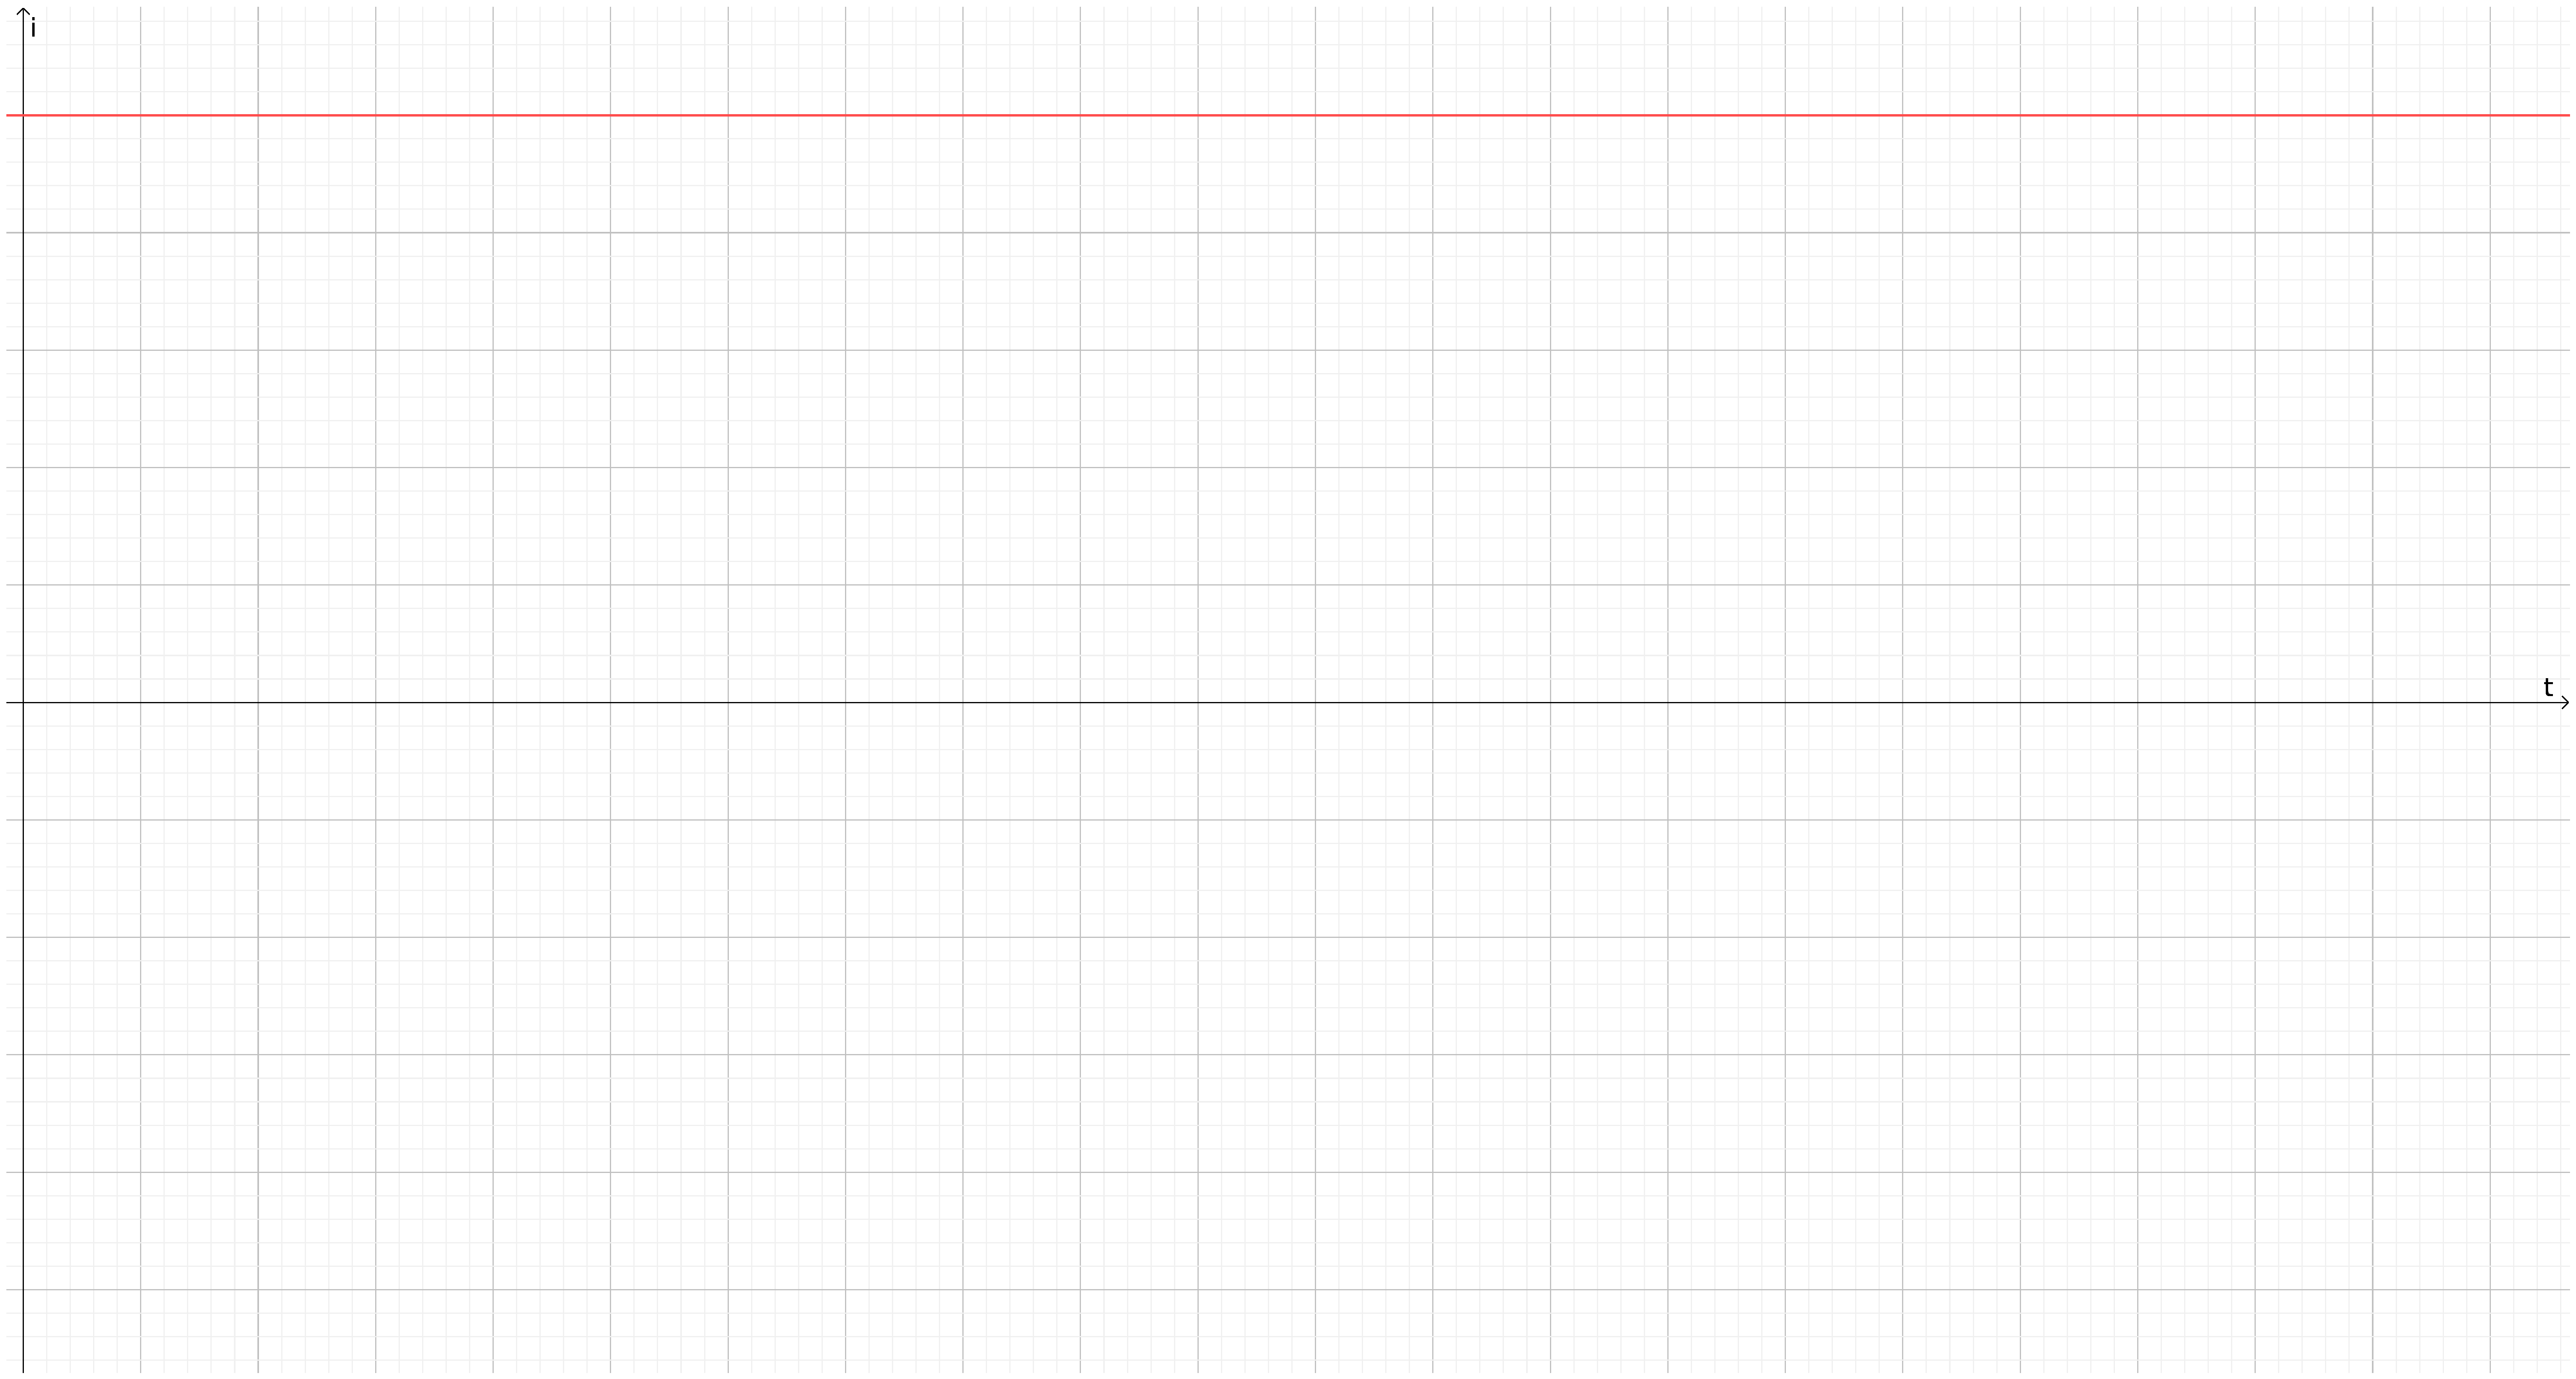
\includegraphics[width=0.45\textwidth]{DirCur.eps}
        \hspace{0.09\textwidth}
        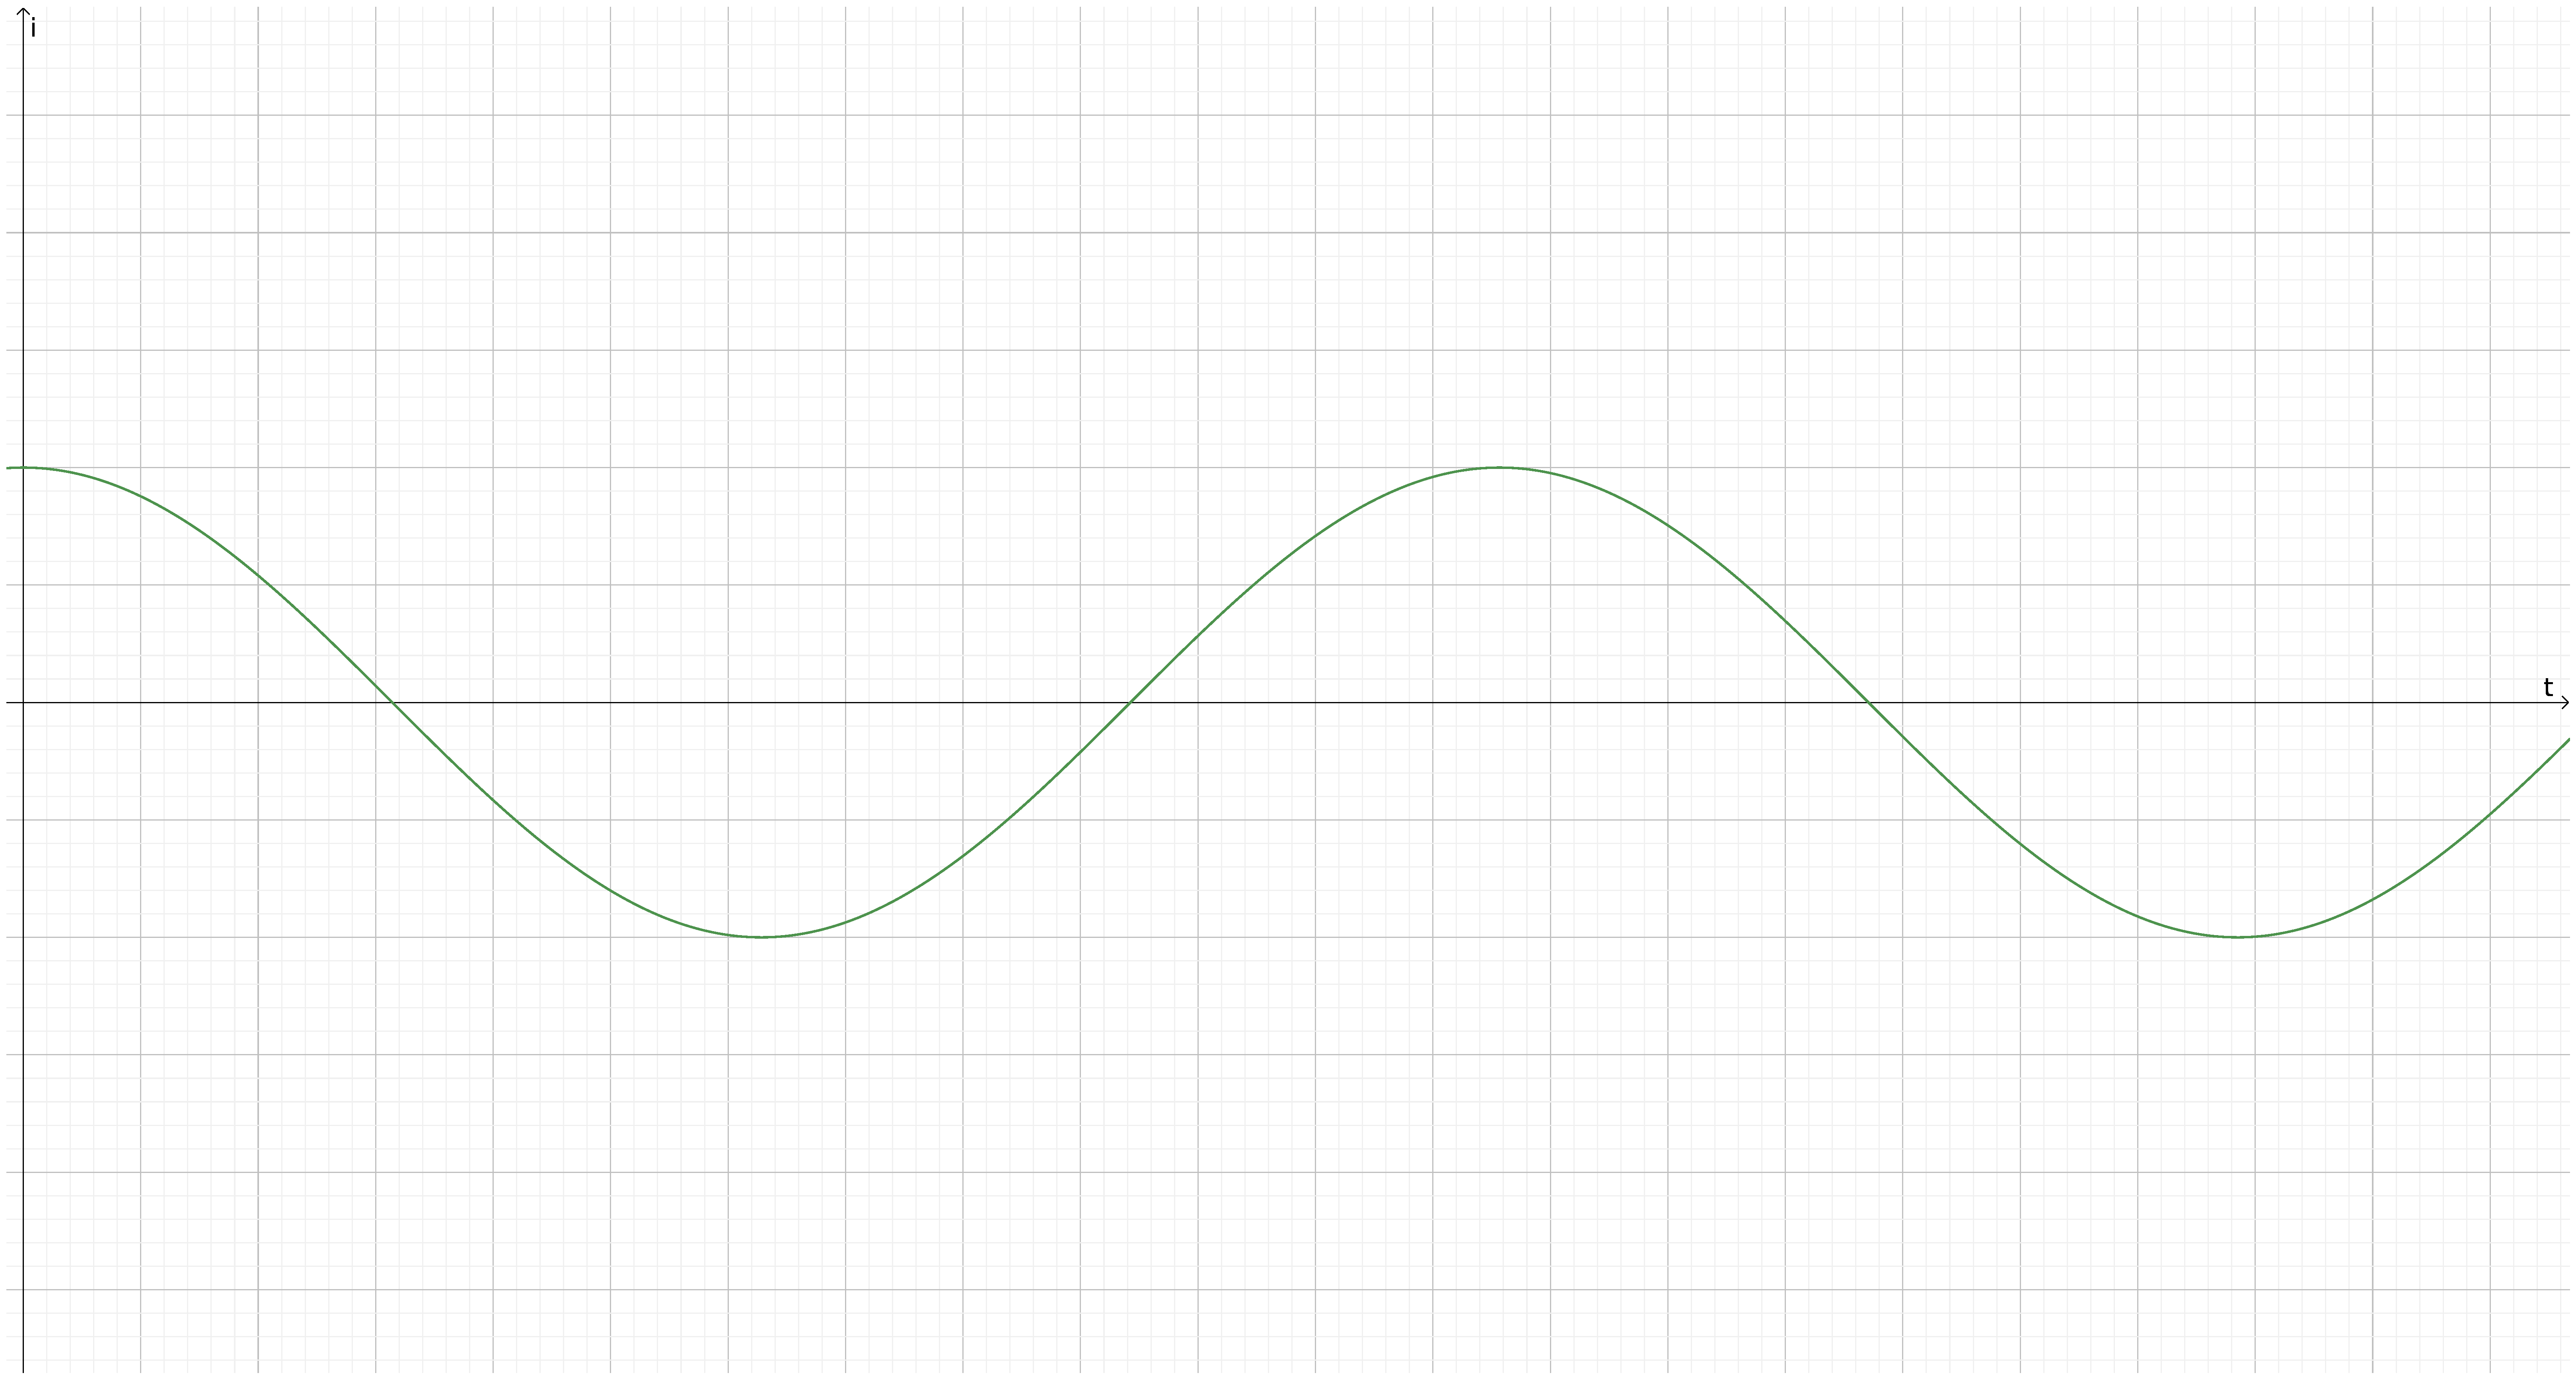
\includegraphics[width=0.45\textwidth]{AltCur.eps}
        \caption{Direct and Alternating Current}
    \end{figure}
    \subsubsection{Notation for Current}
    \subsection{Voltage}
    Voltage is the energy transferred to or from a circuit element per unit of charge that flows through it. 
    $$V(t)=\frac{dw(t)}{dq(t)}$$
    Voltage is often thought of as the potential difference across a circuit element. The polarity of the voltage is used to determine which node of a circuit element is at a higher potential then the other. If a circuit element has two nodes $a$ and $b$ with a voltage $V$ across it such that $a$ is the negative terminal and $b$ is the positive terminal then it can be said that $b$ is $V$ volts higher in potential then $a$. For analysis purposes, reference polarities can be assigned if they are not given. The reference polarities can be chosen arbitrarily and if the actual polarity is the opposite the value of $V$ is negative. 
    \subsection{Ideal Circuit Elements:}
    All circuit elements are characterized by the voltage current relationship they hold.
    \subsubsection{Ideal Conductor:}
    An ideal conductor is a conductor with $0$ resistance; this implies that the current through the conductor stays constant, and there is $0$ voltage drop across the conductor, or $R=0\Omega$, $\Delta i=0A$, and $V=0V$. The components on either side of the conductor are treated as if they are shorted (connected) together. The absence of a conductor is an open circuit. Since all conductors are ideal, they can be as arbitrarily long or short as necessary as long as the connection remains the same. 
    \subsubsection{Sources:}
    \begin{enumerate}
        \item Independent Voltage Sources:\\
        Tells which terminal is at a higher potential voltage and by what amount. The current is unknown and is dependent on the circuit the voltage source is connected to. A voltage source can be either AC or DC
        \item Dependent Voltage Source:\\
        The voltage provided by a dependent voltage source is based on some other value in the circuit. The voltage current characteristics are the same as a independent voltage source, except the value of the voltage provided depends on a voltage or current elsewhere in the circuit. 
        \item Independent Current Source:\\
        Tells the exact value of the current flowing through it. The current provided is unaffected by other elements in the circuit, but the voltage is dependent on the circuit connected to the source.
        \item Dependent Current Source:\\
        A dependent current source has the same properties as an independent current source except the current is dependent on the current or voltage in another element of the circuit.
    \end{enumerate} 
    \subsection{Resistors}
    Resistors resist the flow of current by 
    \section{Resistive Circuits}
    \section{Operational Amplifiers}
    \section{Capacitors and Inductors}
    \section{Sinusoidal Currents and Voltages}
    \section{DC Machines}  
\end{document}